\documentclass[border=8pt]{standalone}
\usepackage{tikz}
\usetikzlibrary{arrows.meta,positioning,calc,backgrounds,fit}

\definecolor{ink}{HTML}{263238}
\definecolor{acc}{HTML}{1565C0}
\definecolor{gateB}{HTML}{D84315}
\definecolor{gateC}{HTML}{6A1B9A}
\definecolor{ctrl}{HTML}{00695C}
\definecolor{pass}{HTML}{43A047}
\definecolor{fail}{HTML}{E53935}
\definecolor{lite}{HTML}{ECEFF1}

\begin{document}
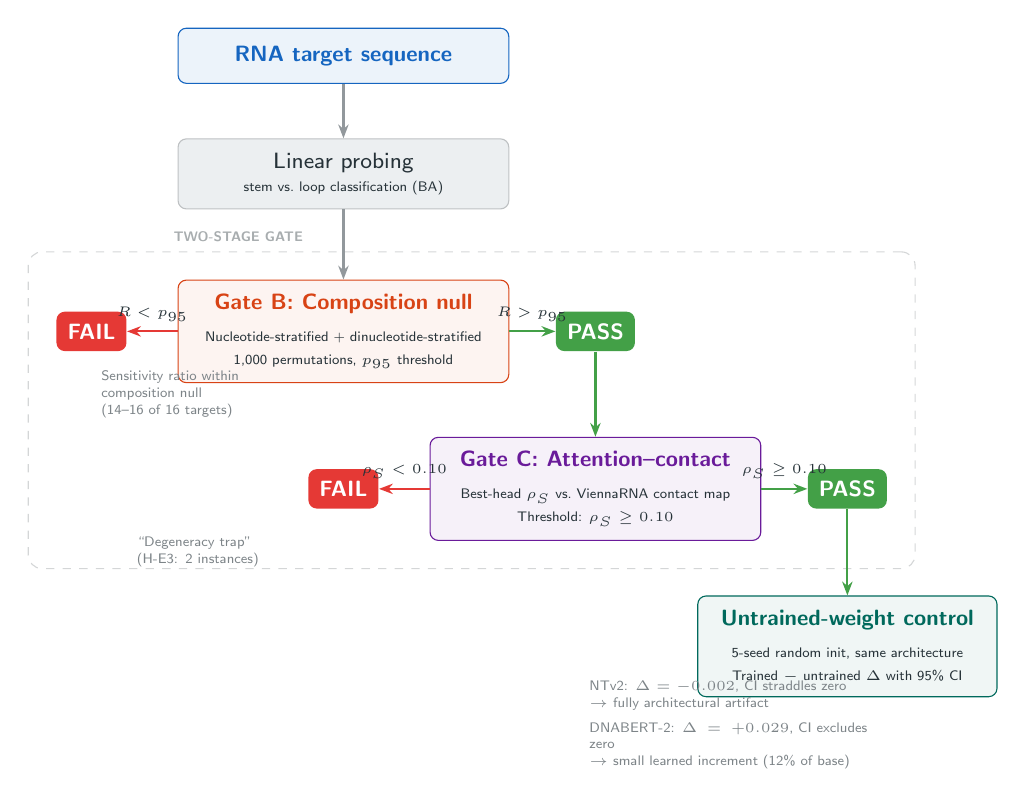
\begin{tikzpicture}[
    >={Stealth[length=5pt]},
    every node/.style={font=\sffamily\small, text=ink},
    box/.style={draw=ink!30, fill=white, rounded corners=3pt,
        minimum height=0.7cm, minimum width=4.2cm, inner sep=5pt,
        font=\sffamily\footnotesize, align=center},
    gatebox/.style={box, minimum height=1.2cm, minimum width=4.2cm},
    tag/.style={font=\sffamily\tiny\bfseries, text=white,
        fill=#1, rounded corners=2pt, inner sep=2pt},
    verdict/.style={font=\sffamily\footnotesize\bfseries, rounded corners=3pt,
        minimum height=0.5cm, inner sep=4pt},
    annot/.style={font=\sffamily\tiny, text=ink!60, text width=3.8cm, anchor=west},
]

% Input
\node[box, fill=acc!8, draw=acc, text=acc, font=\sffamily\footnotesize\bfseries]
    (inp) at (0, 0) {RNA target sequence};

% Probing
\node[box, fill=lite] (probe) at (0, -1.5) {Linear probing\\[-1pt]
    {\tiny stem vs.\ loop classification (BA)}};

% Arrow
\draw[->, thick, ink!50] (inp) -- (probe);

% Gate B
\node[gatebox, fill=gateB!6, draw=gateB] (gb) at (0, -3.5)
    {\textbf{\textcolor{gateB}{Gate B: Composition null}}\\[2pt]
    {\tiny Nucleotide-stratified + dinucleotide-stratified}\\[-1pt]
    {\tiny 1{,}000 permutations, $p_{95}$ threshold}};

\draw[->, thick, ink!50] (probe) -- (gb);

% Gate B outcomes
\node[verdict, fill=fail, text=white] (gb_fail) at (-3.2, -3.5) {FAIL};
\node[annot] at (-3.2, -4.3) {Sensitivity ratio within\\composition null\\(14--16 of 16 targets)};

\node[verdict, fill=pass, text=white] (gb_pass) at (3.2, -3.5) {PASS};

\draw[->, thick, fail] (gb) -- (gb_fail) node[midway, above, font=\sffamily\tiny] {$R < p_{95}$};
\draw[->, thick, pass] (gb) -- (gb_pass) node[midway, above, font=\sffamily\tiny] {$R > p_{95}$};

% Gate C
\node[gatebox, fill=gateC!6, draw=gateC] (gc) at (3.2, -5.5)
    {\textbf{\textcolor{gateC}{Gate C: Attention--contact}}\\[2pt]
    {\tiny Best-head $\rho_S$ vs.\ ViennaRNA contact map}\\[-1pt]
    {\tiny Threshold: $\rho_S \geq 0.10$}};

\draw[->, thick, pass] (gb_pass) -- (gc);

% Gate C outcomes
\node[verdict, fill=fail, text=white] (gc_fail) at (0, -5.5) {FAIL};
\node[annot, anchor=east, text width=2.5cm] at (0, -6.3)
    {``Degeneracy trap''\\(H-E3: 2 instances)};

\node[verdict, fill=pass, text=white] (gc_pass) at (6.4, -5.5) {PASS};

\draw[->, thick, fail] (gc) -- (gc_fail) node[midway, above, font=\sffamily\tiny] {$\rho_S < 0.10$};
\draw[->, thick, pass] (gc) -- (gc_pass) node[midway, above, font=\sffamily\tiny] {$\rho_S \geq 0.10$};

% Untrained-weight control
\node[gatebox, fill=ctrl!6, draw=ctrl, minimum width=3.8cm] (uc) at (6.4, -7.5)
    {\textbf{\textcolor{ctrl}{Untrained-weight control}}\\[2pt]
    {\tiny 5-seed random init, same architecture}\\[-1pt]
    {\tiny Trained $-$ untrained $\Delta$ with 95\% CI}};

\draw[->, thick, pass] (gc_pass) -- (uc);

% UC annotation
\node[annot] at (3.0, -8.5)
    {NTv2: $\Delta = -0.002$, CI straddles zero\\
    $\to$ fully architectural artifact\\[3pt]
    DNABERT-2: $\Delta = +0.029$, CI excludes zero\\
    $\to$ small learned increment (12\% of base)};

% Dashed box around the two-stage gate
\begin{scope}[on background layer]
\node[draw=ink!20, dashed, rounded corners=5pt, inner sep=10pt,
    fit=(gb)(gb_fail)(gb_pass)(gc)(gc_fail)(gc_pass),
    label={[font=\sffamily\tiny\bfseries, text=ink!40]above left:TWO-STAGE GATE}] {};
\end{scope}

\end{tikzpicture}
\end{document}
